\noindent El capitulo incluye información relacionada con las tecnologías utilizadas en el proyecto, el entorno de trabajo y los datos. En la Sección \ref{sec:sistema} se describe el concepto de \gls{API}, una de las fuentes de datos en crudo y la estructura del modelo. A continuación, la Sección \ref{sec:dataset} está destinada al montaje del laboratorio de análisis de muestras \textit{ransomware}. La Sección \ref{sec:reports} incluye el proceso de construcción del conjunto de datos final, incluyendo información de la estructura de los reportes obtenidos en el análisis y las pautas seguidas para la limpieza y la extracción de características. Por último, en la Sección \ref{sec:model} se detallan el modelo y los algoritmos utilizados, así como librerías importantes para la construcción del mismo.

\section{Descripción del Sistema Propuesto} \label{sec:sistema}

\noindent El objetivo del sistema propuesto es la detección de ransomware mediante la extracción de las llamadas a la \gls{API} de Windows, utilizando algoritmos supervisados de aprendizaje automático para construir un modelo de clasificación que detecte si un archivo es ransomware o no.



Una \gls{API} (interfaz de programación de aplicaciones) proporciona una abstracción para un problema y especifica cómo los clientes deben interactuar con los componentes software para implementar una solución. Suelen ser distribuidas como librerías software, definiendo bloques de desarrollo reusables que permiten añadir funcionalidades en múltiples aplicaciones \cite{reddy2011api}. 

Microsoft suministra a los desarrolladores de Windows una \gls{API} documentada profesionalmente para facilitar el proceso de creación de una aplicación. Ésta provee todas las funcionalidades básicas y permite el despliegue de entornos ricos e interactivos. De manera análoga, una aplicación de Windows puede ser mapeada y explicada por las llamadas a la {API} que realice, entendiendo así su comportamiento. Por ejemplo, si el proceso llama a la función \textit{WriteFile}, se puede saber que se va a escribir en un fichero del sistema. Si se invoca, por ejemplo a \textit{CryptEncrypt}, la aplicación va a efectuar un cifrado en nuestro sistema de ficheros. Este tipo de llamadas pueden ser muy útiles para la detección de ransomware de cifrado, aunque aplicaciones benignas también lo utilicen. Para este estudio, se han recogido un total de 302 llamadas distintas a la \gls{API} de Windows, realizando una distinción en la recogida de datos: se conforma un \textit{dataset} en el que, de manera binaria, un proceso a invocado a la función de sistema correspondiente, y otro que señala la cantidad de llamadas totales para cada función \cite{10.1145/1654988.1655003}.


Los datos utilizados en el proyecto se han obtenido de dos formas diferentes. Primero, el grupo de investigación GASS \cite{GASS01} proporcionó 21 muestras de \textit{ransomware} para su análisis en un entorno controlado, como se explica en la Sección \ref{sec:lab}. Por otro lado, el grupo GASS \cite{GASS01} ha desarrollado una herramienta con la que se accede a un número elevado de muestras, extrayendo múltiples informes obtenidos de análisis realizados en la página web de Cuckoo Sandbox por usuarios anónimos. De esta forma se obtiene un fichero en formato .json con información de 5435 muestras de \textit{ransomware} y otro fichero con información de 10896 muestras de \textit{goodware} (software benigno). Combinando ambos métodos, es posible componer un conjunto de datos inicial de gran extensión y mayor variedad. El análisis de las muestras y la extracción de las características relevantes se explica con más detalle en la Sección \ref{sec:reports}. Finalmente, los resultados obtenidos del análisis se usarán para entrenar al modelo de \gls{ML}.
La Figura \ref{fig:fase1} muestra el proceso en términos generales.

\begin{figure}[h!]
\begin{center}
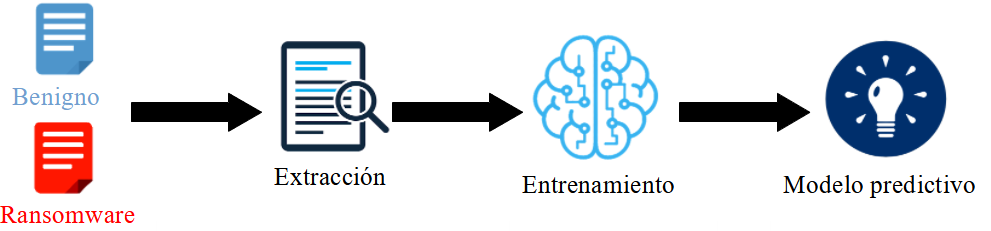
\includegraphics[width=1\linewidth]{images/fase1.png}
\end{center}
\caption{Extracción de características y creación del modelo predictivo.}
\label{fig:fase1} 
\end{figure}

A partir del entrenamiento se creará un modelo predictivo que podrá decir si archivo es ransomware o benigno. En la fase de predicción se hace uso del modelo predictivo para sacar inferencias, y este proceso es similar al de entrenamiento, ya que ambos comienzan extrayendo características. Sin embargo, esta vez en lugar de entrenar el modelo usando esas características, se predecirá la naturaleza del archivo desconocido. El desarrollo del modelo y los algoritmos de aprendizaje automático usados se detallan en la Sección \ref{sec:algoritmos}. 
La Figura \ref{fig:fase2} muestra este proceso.

\begin{figure}[h!]
\begin{center}
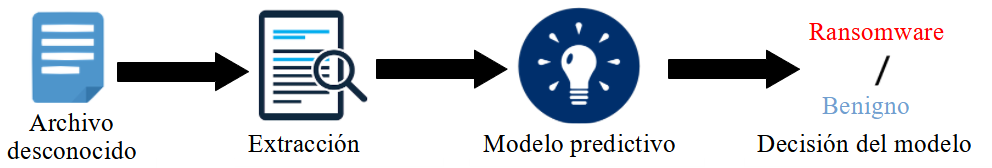
\includegraphics[width=1\linewidth]{images/fase2.png}
\end{center}
\caption{Clasificación de un archivo con un modelo predictivo.}
\label{fig:fase2} 
\end{figure}


La Figura \ref{fig:sistema} representa el diagrama de flujo del sistema propuesto en este trabajo, siguiendo los pasos detallados a continuación:
\begin{enumerate}
    \item Obtención de muestras ransomware y benignas e información de reportes.
    \item Ejecución y análisis de las muestras en un entorno controlado usando Cuckoo Sandbox.
    \item Unión y limpieza de los datos, extracción de características y \textit{dataset}.
    \item División del \textit{dataset} en datos de entrenamiento y datos de prueba.
    \item Entrenamiento del modelo.
    \item Utilización del modelo.
    \item Salida del modelo y clasificación de la muestra.
    \item Análisis, generación de gráficas y conclusiones.
\end{enumerate}

\begin{figure}[h!]
\begin{center}
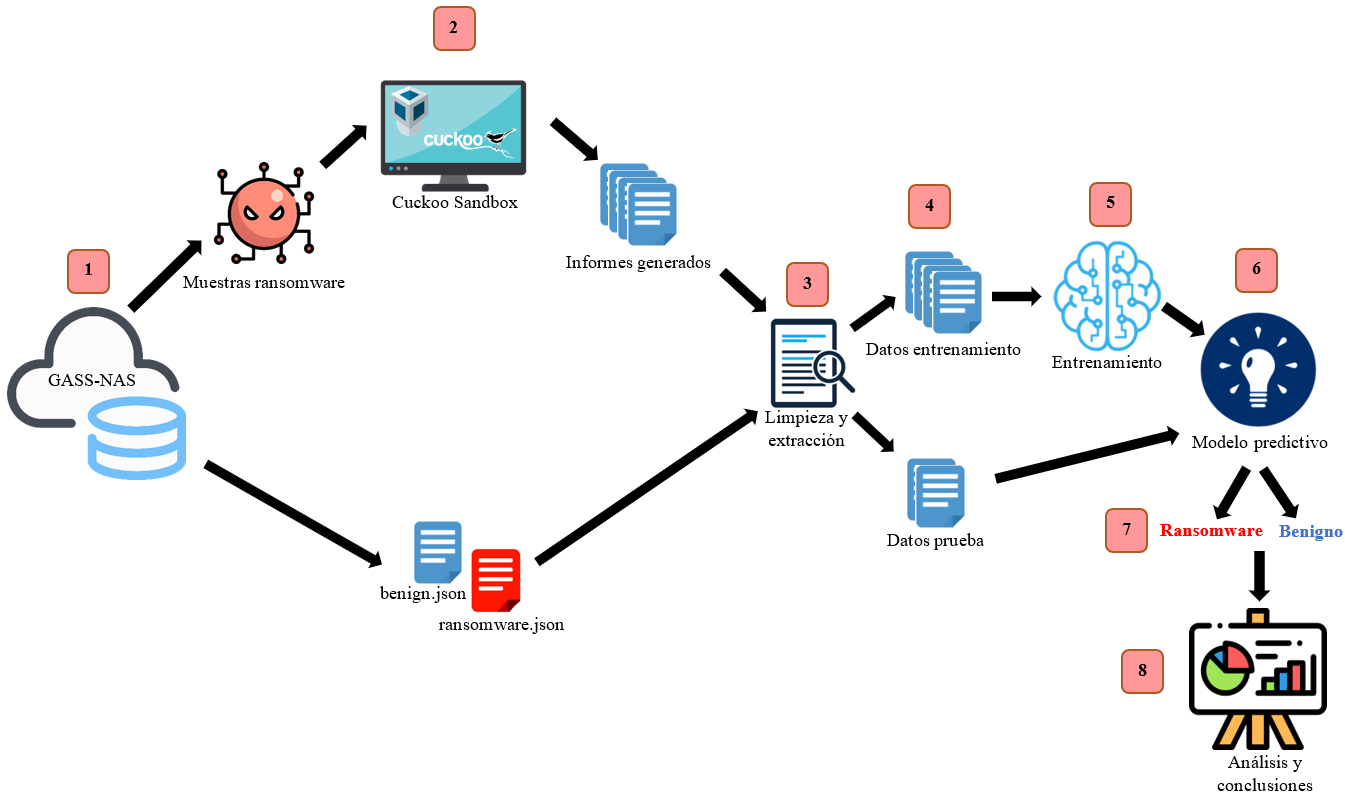
\includegraphics[width=1\linewidth]{images/sistemapropuesto.PNG}
\end{center}
\caption{Diagrama de flujo del sistema propuesto.}
\label{fig:sistema} 
\end{figure}



\section{Entorno de Obtención de Datos} \label{sec:dataset}

\noindent A la hora de ejecutar muestras reales de \textit{ransomware} para su análisis, se puede causar daño al sistema con borrado de archivos, cambios en los registros y robo de información confidencial, entre otras cosas. Para evitar esto, es preciso contar con un entorno seguro donde ejecutar el malware sin poner en riesgo los equipos o la red \cite{CMA}.

Cuckoo Sandbox es una herramienta de análisis automatizado de malware de código abierto en Windows, macOS, Linux y Android. Esta herramienta utiliza la tecnología de \textit{sandboxing}, que, en terminología informática, es una técnica que consiste en aislar la ejecución de un programa no fiable o malicioso llevándola a un entorno seguro que no comprometa el sistema, de forma que se puedan analizar las actividades del malware sin preocupación por los cambios que realice el proceso maligno.

Existen múltiples herramientas que utilicen \textit{sandboxing} y permitan construir un laboratorio de análisis de malware, entre ellas, Buster Sandbox Analyzer, Zero Wine o Malheur, pero en este trabajo se recurre a Cuckoo Sandbox debido a que es la más completa y, siendo de código abierto y teniendo un diseño modular, permite personalizar cualquier aspecto del procesamiento del análisis de los resultados, de la generación de informes y del entorno de análisis. Además, tiene una guía detallada de los requisitos para integrar la herramienta con el sistema.

Cuckoo Sandbox, se inició como un proyecto de verano parte del programa Google Summer of Code en 2010, lanzando la primera beta en febrero de 2011. El diseñador y desarrollador de Cuckoo, Claudio Guarnieri, es aún el principal coordinador del proyecto. En marzo de 2012, Cuckoo Sandbox ganó la primera ronda del programa Magnificent7 organizado por Rapid7 (un importante sistema de Gestión de Vulnerabilidades y análisis de \textit{endpoints}, con más  de 20 años de trayectoria). Esta herramienta fue mejorando y obteniendo méritos hasta febrero de 2016, cuando la versión 2.0 fue publicada, siendo esta una versión muy completa y adaptada al uso diario.

La arquitectura de Cuckoo se muestra en la Figura \ref{fig:Diagrama}. Consiste en un software central que maneja la ejecución y el análisis de muestras, en el caso de este proyecto, ejecutando cada una en una máquina virtual aislada. De esta forma, los componentes principales de la infraestructura del laboratorio de análisis de malware (y por lo tanto de Cuckoo Sandbox) son una máquina anfitrión que gestiona el proceso de análisis, la cual tendrá acceso a Internet, y un número de máquinas virtuales conectadas a una red virtual donde las muestras de malware se ejecutan de forma segura y aislada para ser analizadas.

\begin{figure}[!htb]
\begin{center}
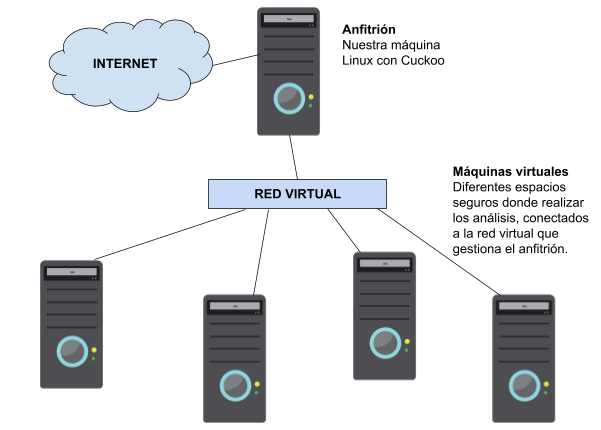
\includegraphics[width=0.9\linewidth]{images/infraestructuracuckoo.png}
\end{center}
\caption{Arquitectura de Cuckoo Sandbox}
\label{fig:Diagrama}
\end{figure}

Hay otra manera de utilizar Cuckoo Sandbox sin necesidad de una máquina virtual propia, y es mediante el uso de la interfaz web de la herramienta (\href{https://cuckoo.cert.ee/}{Cuckoo Sandbox Online}). La ventaja de este método es que no es necesario construir un laboratorio de análisis con Cuckoo descargado, ya que es accesible mediante Internet. Pero tiene un gran inconveniente, y es la lentitud del análisis, ya que es necesario subir los archivos manualmente uno por uno y si la página web tiene mucha afluencia, el análisis tardará más. Por esta razón se decidió construir un laboratorio de análisis propio en una máquina con el sistema operativo recomendado por los autores de Cuckoo Sandbox, que es Linux con distribución Ubuntu 18.04.5 \gls{LTS}.

\subsection{Laboratorio de análisis} \label{sec:lab}
%anexo a
\label{anexo-a}
\noindent Una vez entendido el concepto de \textit{sandboxing}, y la necesidad de construir un laboratorio de análisis de malware para el trabajo, comienza la preparación del mismo.

La máquina anfitrión será un ordenador con sistema operativo Linux, utilizando la distribución Ubuntu en la versión 18.04.5 \gls{LTS}.

Se necesitan una serie de requisitos para la instalación y el correcto funcionamiento de Cuckoo.

Será necesario tener la versión adecuada de Python (actualmente soporta Python 2.7) e instalar una serie de bibliotecas:

\begin{listing}[style=consola, numbers=none]
$ sudo apt-get install python python-pip python-dev libffi-dev libssl-dev
$ sudo apt-get install python-virtualenv python-setuptools
$ sudo apt-get install libjpeg-dev zlib1g-dev swig
\end{listing}

Para poder utilizar la interfaz web Django y PostgreSQL como base de datos, se necesita MongoDB y PostgreSQL:

\begin{listing}[style=consola, numbers=none]
$ sudo apt-get install mongodb
$ sudo apt-get install postgresql libpq-dev
\end{listing}

Las máquinas virtuales basadas en Windows 7 donde se ejecutarán las muestras de malware serán generadas a través de VirtualBox, un software de virtualización muy completo el cual está soportado por Cuckoo, aunque se puede utilizar otro software de virtualización. En este caso se utiliza la versión 5.2.42 de VirtualBox, la cual se puede descargar e instalar desde la página oficial o utilizando los comandos siguientes:

\begin{listing}[style=consola, numbers=none]
$ echo deb http://download.virtualbox.org/virtualbox/debian xenial contrib | sudo \
tee -a /etc/apt/sources.list.d/virtualbox.list
$ wget -q https://www.virtualbox.org/download/oracle_vbox_2016.asc -O- | sudo \
apt-key add -
$ sudo apt-get update
$ sudo apt-get install virtualbox-5.2
\end{listing}

Para poder obtener información de la actividad de red del malware se recurre a tcpdump, que rastreará la red para capturar el tráfico a la hora de analizar una muestra.

\begin{listing}[style=consola, numbers=none]
$ sudo apt-get install tcpdump apparmor-utils
\end{listing}

Esta herramienta necesita privilegios de superusuario, los cuales les serán otorgados únicamente a ella y no a Cuckoo Sandbox:

\begin{listing}[style=consola, numbers=none]
$ sudo groupadd pcap

$ sudo usermod -a -G pcap (nombre_usuario)
$ sudo chgrp pcap /usr/sbin/tcpdump
$ sudo setcap cap_net_raw,cap_net_admin=eip /usr/sbin/tcpdump
$ sudo aa-disable /usr/sbin/tcpdump
\end{listing}

Tras esto, se instala M2crypto, un módulo de Python que será necesario para el análisis de muestras:

\begin{listing}[style=consola, numbers=none]
$ sudo pip install m2crypto
\end{listing}

En este caso, se utiliza VirtualBox y será necesario incluir al usuario con el que se ejecuta Cuckoo en el grupo ``vboxusers'', para que Cuckoo pueda identificar las máquinas virtuales:

\begin{listing}[style=consola, numbers=none]
$ sudo usermod -a -G vboxusers (nombre_usuario)
\end{listing}

A continuación, se crea un entorno virtual, para añadir otro factor más de seguridad al laboratorio y en este entorno será donde posteriormente se instale Cuckoo Sandbox y se trabaje. Para ello, descargamos un \href{https://gist.github.com/jstrosch/de20131dda2aac5cd1116dd44b8f2474#file-cuckoo-setup-virtualenv-sh}{\textcolor{blue}{script bash de GitHub}} el cual sirve para instalar esta funcionalidad: 

\begin{listing}[style=consola, numbers=none]
$ sudo -u <USERNAME> cuckoo-setup-virtualenv.sh
\end{listing}

Una vez instalada esta herramienta, se crea un entorno virtual, en el caso de este trabajo se le ha dado el nombre de ``cuckoo-test'' y llegados a este punto, siempre se trabajará dentro de este entorno, por lo que será muy importante asegurarse de que estamos dentro del entorno virtual al utilizar un terminal.


\begin{listing}[style=consola, numbers=none]
$ mkvirtualenv -p python2.7 cuckoo-test
\end{listing}

Tras la ejecución del comando anterior, se estará trabajando dentro de un entorno virtual donde se realizan el resto de pasos. Primero se requiere la actualización de los módulos pip y setuptools y después, se procede a la instalación de Cuckoo:

\begin{listing}[style=consola, numbers=none]
(cuckoo-test) $ pip install -U pip setuptools
(cuckoo-test) $ pip install -U cuckoo
\end{listing}

A continuación, se deberá descargar una ISO de Windows 7 y se monta: \cite{HATCHING}

\begin{listing}[style=consola, numbers=none]
(cuckoo-test) $ wget https://cuckoo.sh/win7ultimate.iso
(cuckoo-test) $ mkdir /mnt/win7
(cuckoo-test) $ sudo mount -o ro,loop win7ultimate.iso /mnt/win7
\end{listing}

Para gestionar la creación de máquinas virtuales para Cuckoo, el software que usan y la captura de estados, el uso de la herramienta VMCloak facilitará estas tareas ya que está diseñada para crear máquinas virtuales que Cuckoo Sandbox pueda utilizar. \cite{VMCLOAK} Es necesario instalar algunos paquetes previos para la correcta integración con Cuckoo, y después instalar VMCloak: \cite{HATCHING}

\begin{listing}[style=consola, numbers=none]
(cuckoo-test) $sudo apt-get -y install build-essential libssl-dev libffi-dev \ 
python-dev genisoimage
(cuckoo-test) $ sudo apt-get -y install zlib1g-dev libjpeg-dev
(cuckoo-test) $ sudo apt-get -y install python-pip python-virtualenv \ 
python-setuptools swig

(cuckoo-test) $ pip install -U vmcloak
\end{listing}

Una vez la herramienta está instalada, se crea una interfaz de red a la que se conectarán las máquinas virtuales, se configura la ISO montada previamente con las características adecuadas (en este caso, serán máquinas virtuales con 2 CPUs y una memoria RAM de 2048MB) utilizando los siguientes comandos: \cite{HATCHING}

\begin{listing}[style=consola, numbers=none]
(cuckoo-test) $ vmcloak-vboxnet0 
(cuckoo-test) $ vmcloak init --verbose --win7x64 win7x64base --cpus 2 --ramsize 2048
\end{listing}

El siguiente paso es instalar el software necesario, que una vez creados los estados de la imagen, no se podrá modificar, por eso, el primer paso será clonar la máquina en su versión original vacía, para instalar software ahí y guardar los estados. 
Entre el software que necesario para las máquinas encontramos java, adobepdf, flash y pillow (este último será el paquete que realice capturas de pantalla durante el análisis del malware): \cite{HATCHING}

\begin{listing}[style=consola, numbers=none]
(cuckoo-test) $ vmcloak clone win7x64base cuckooVM
(cuckoo-test) $ vmcloak install cuckooVM adobepdf dotnet java flash vcredist \ 
vcredist.version=2015u3 wallpaper
(cuckoo-test) $ vmcloak install cuckooVM pillow
\end{listing}

Llegados a este punto, se crean los estados de la máquina virtual. Dadas las características del equipo en el que se está construyendo el laboratorio de análisis de malware, se crean 3 estados, lo que permitirá realizar un máximo de 3 análisis simultáneos. Con el siguiente comando, se crearán 3 máquinas virtuales con IPs 192.168.56.101, 192.168.56.102 y 192.168.56.103: \cite{HATCHING}

\begin{listing}[style=consola, numbers=none]
(cuckoo-test) $ vmcloak snapshot --count 3 cuckooVM 192.168.56.101
\end{listing}

Con todo lo realizado hasta ahora, el laboratorio está casi preparado y únicamente quedaría configurar Cuckoo Sandbox para ponerlo a funcionar. Para ello es necesario iniciar cuckoo, que mostrará por defecto el directorio de trabajo ``\verb!/home/nombre_usuario/.cuckoo!'', este directorio se podrá modificar sin problema, aunque en el caso de este proyecto, se trabajará en el definido por defecto. 

\begin{listing}[style=consola, numbers=none]
(cuckoo-test) $ cuckoo init
(cuckoo-test) $ cuckoo community
\end{listing}

También será necesario modificar los ficheros de configuración de Cuckoo, que se encuentran en la carpeta ``\verb!conf!'' dentro del directorio principal de trabajo, personalizando los ajustes y configurando las máquinas virtuales.

En primer lugar, la edición del fichero ``\verb!virtualbox.conf!'' que contiene opciones sobre el software de virtualización, en este caso, se edita el campo ``\verb!mode!'' que por defecto tendrá el valor ``\verb!headless!'' y pone el valor ``\verb!gui!''. Este cambio permitirá ver la máquina virtual en ejecución cuando se realice un análisis, si por el contrario se quiere ver únicamente el resultado final y no lo que va sucediendo, se mantendrá el valor ``\verb!headless!''. El fichero quedaría de la siguiente manera:

\lstset{language=bash,breaklines=true, basicstyle=\footnotesize}
\begin{lstlisting}[frame=single, caption=Fichero ``virtualbox.conf'']
[virtualbox]
# Specify which VirtualBox mode you want to run your machines on.
# Can be "gui" or "headless". Please refer to VirtualBox's official
# documentation to understand the differences.
mode = gui
\end{lstlisting}

Con el siguiente comando, que modificará el fichero anterior, se añaden las máquinas virtuales creadas a Cuckoo con su configuración. \cite{HATCHING}

\begin{listing}[style=consola, numbers=none]
(cuckoo-test) $ while read -r vm ip; do cuckoo machine --add $vm $ip; 
done < <(vmcloak list vms)
\end{listing}

El resultado del fichero será el siguiente:

\break

\lstset{language=bash,breaklines=true, basicstyle=\footnotesize}
\begin{lstlisting}[frame=single, caption=Fichero ``virtualbox.conf'', breaklines=true]
[192.168.56.1011]
# Specify the label name of the current machine as specified in your
# VirtualBox configuration.
label = 192.168.56.1011

# Specify the operating system platform used by current machine
# [windows/darwin/linux].
platform = windows

# Specify the IP address of the current virtual machine. Make sure that the
# IP address is valid and that the host machine is able to reach it. If not,
# the analysis will fail.
ip = 192.168.56.101

# (Optional) Specify the snapshot name to use. If you do not specify a
# snapshot name, the VirtualBox MachineManager will use the current snapshot
# Example (Snapshot1 is the snapshot name):
snapshot = 

# (Optional) Specify the name of the network interface that should be used
# when dumping network traffic from this machine with tcpdump. If specified,
# overrides the default interface specified in auxiliary.conf
# Example (vboxnet0 is the interface name):
interface = 

# (Optional) Specify the IP of the Result Server, as your virtual machine 
# sees it.
# The Result Server will always bind to the address and port specified in
# cuckoo.conf, however you could set up your virtual network to use NAT/PAT,
# so you can specify here the IP address for the Result Server as your 
# machine sees it. If you don't specify an address here, the machine will 
# use the default value from cuckoo.conf.
# NOTE: if you set this option you have to set result server IP to 0.0.0.0 
# in cuckoo.conf.
# Example:
resultserver_ip = 192.168.56.1
# (Optional) Specify the port for the Result Server, as your virtual machine
# sees it. The Result Server will always bind to the address and port 
# specified in cuckoo.conf, however you could set up your virtual network 
# to use NAT/PAT, so you can specify here the port for the Result Server as 
# your machine sees it. If you don't specify a port here, the machine will 
# use the default value from cuckoo.conf.
# Example:
resultserver_port = 0
# (Optional) Set your own tags. These are comma separated and help to
# identify specific VMs. You can run samples on VMs with tag you require.
tags = 
# Mostly unused for now. Please don't fill it out.
options = 
# (Optional) Specify the OS profile to be used by volatility for this
# virtual machine. This will override the guest_profile variable in
# memory.conf which solves the problem of having multiple types of VMs
# and properly determining which profile to use.
osprofile = 

[192.168.56.1012]
.
.
. 
\end{lstlisting}

Hecho esto, se quiere dar acceso a Internet a las máquinas de análisis y para ello, es necesario activar la redirección de paquetes (\textit{forwarding}) en la interfaz creada para VirtualBox y en la interfaz de salida (que en este caso es ``wlo1'', pero puede ser ``eth0'' u otra, dependiendo del sistema).

La conexión a Internet es importante para que las muestras de malware muestren su comportamiento completo en los análisis, ya que que se conecten a la red es algo básico en la mayoría de ellas \cite{HATCHING}:

\begin{listing}[style=consola, numbers=none]
(cuckoo-test) $ sudo sysctl -w net.ipv4.conf.vboxnet0.forwarding=1
(cuckoo-test) $ sudo sysctl -w net.ipv4.conf.wlo1.forwarding=1
\end{listing}

Otro aspecto a configurar de Cuckoo, es el módulo ``rooter'', que concede a Cuckoo ciertos permisos para trabajar con comandos de red y poder realizar análisis con opciones de encaminamiento y así sacar el máximo partido a análisis:

\begin{listing}[style=consola, numbers=none]
(cuckoo-test) $ cuckoo rooter --sudo --group gonzalo
\end{listing}

Por último, antes de poder iniciar la interfaz web de Cuckoo Sandbox y empezar a realizar análisis, los últimos ficheros que necesitan edición son el fichero ``\verb!routing.conf!'', cambiando el apartado ``\verb!internet!'' con valor ``\verb!none!'' y dándole el nuevo valor ``\verb!wlo1!'' (la interfaz de red) y el fichero ``\verb!reporting.conf!'' cambiando el valor de ``\verb!enabled!'' en el apartado ``\verb!mongodb!'' de ``\verb!no!'' a ``\verb!yes!'' \cite{HATCHING}.

\lstset{language=bash,breaklines=true, basicstyle=\footnotesize}
\begin{lstlisting}[frame=single, caption=Fichero ``routing.conf'']
[routing]
# Network interface that allows a VM to connect to the entire internet, the
# "dirty line" so to say. Note that, just like with the VPNs, this will allow
# malicious traffic through your network. So think twice before enabling it.
# (For example, to use eth0 as dirty line: "internet = eth0").
internet = wlo1
\end{lstlisting}

\lstset{language=bash,breaklines=true, basicstyle=\footnotesize}
\begin{lstlisting}[frame=single, caption=Fichero ``reporting.conf'']
[mongodb]
enabled = yes
host = 127.0.0.1
port = 27017
db = cuckoo
store_memdump = yes
paginate = 100
# MongoDB authentication (optional).
username = 
password = 
\end{lstlisting}

Con el laboratorio puesto a punto, ya es posible realizar el análisis de las muestras para obtener parte de los datos que serán procesados para alimentar el modelo de \gls{ML}. El análisis de una muestra usando Cuckoo Sandbox se detalla en el Anexo \ref{anexo-b}.

%\section{Análisis de una muestra con Cuckoo Sandbox}
%\noindent Configurada la herramienta, se podrán realizar análisis en el laboratorio construido utilizando Cuckoo Sandbox. Para ello, es necesario ejecutar una serie de comandos para iniciar correctamente el entorno cada vez que el sistema sea reiniciado:

\begin{enumerate}
\item En cada terminal que se abra para trabajar, iniciar el entorno virtual “cuckoo-test”: 
\begin{listing}[style=consola, numbers=none]
$ workon cuckoo-test 
\end{listing}
\item Activar forwarding para la interfaz de red:
\begin{listing}[style=consola, numbers=none]
(cuckoo-test) $ sudo sysctl -w net.ipv4.conf.wlo1.forwarding=1
\end{listing}
\item Crear interfaz con VMCloak:
\begin{listing}[style=consola, numbers=none]
(cuckoo-test) $ vmcloak-vboxnet0
\end{listing}
\item Ejecutar Cuckoo Rooter:
\begin{listing}[style=consola, numbers=none]
(cuckoo-test) $ cuckoo rooter --sudo --group gonzalo
\end{listing}
\item Ejecutar Cuckoo:
\begin{listing}[style=consola, numbers=none]
(cuckoo-test) $ cuckoo
\end{listing}
\item Ejecutar Cuckoo Web:
\begin{listing}[style=consola, numbers=none]
(cuckoo-test) $ cuckoo web --host 127.0.0.1 --port 8080
\end{listing}
\end{enumerate}

Una vez ejecutados estos comandos, si se accede en el navegador a la dirección 127.0.0.1:8080 se encontrará la página principal de la interfaz web de Cuckoo Sandbox, como muestra la Figura \ref{fig:DashboardCuckoo}, donde aparece información de la versión de la herramienta, detalles sobre el uso de memoria y otros. Además, desde aquí será posible subir una muestra para su análisis.


\begin{figure}[h!]
\begin{center}
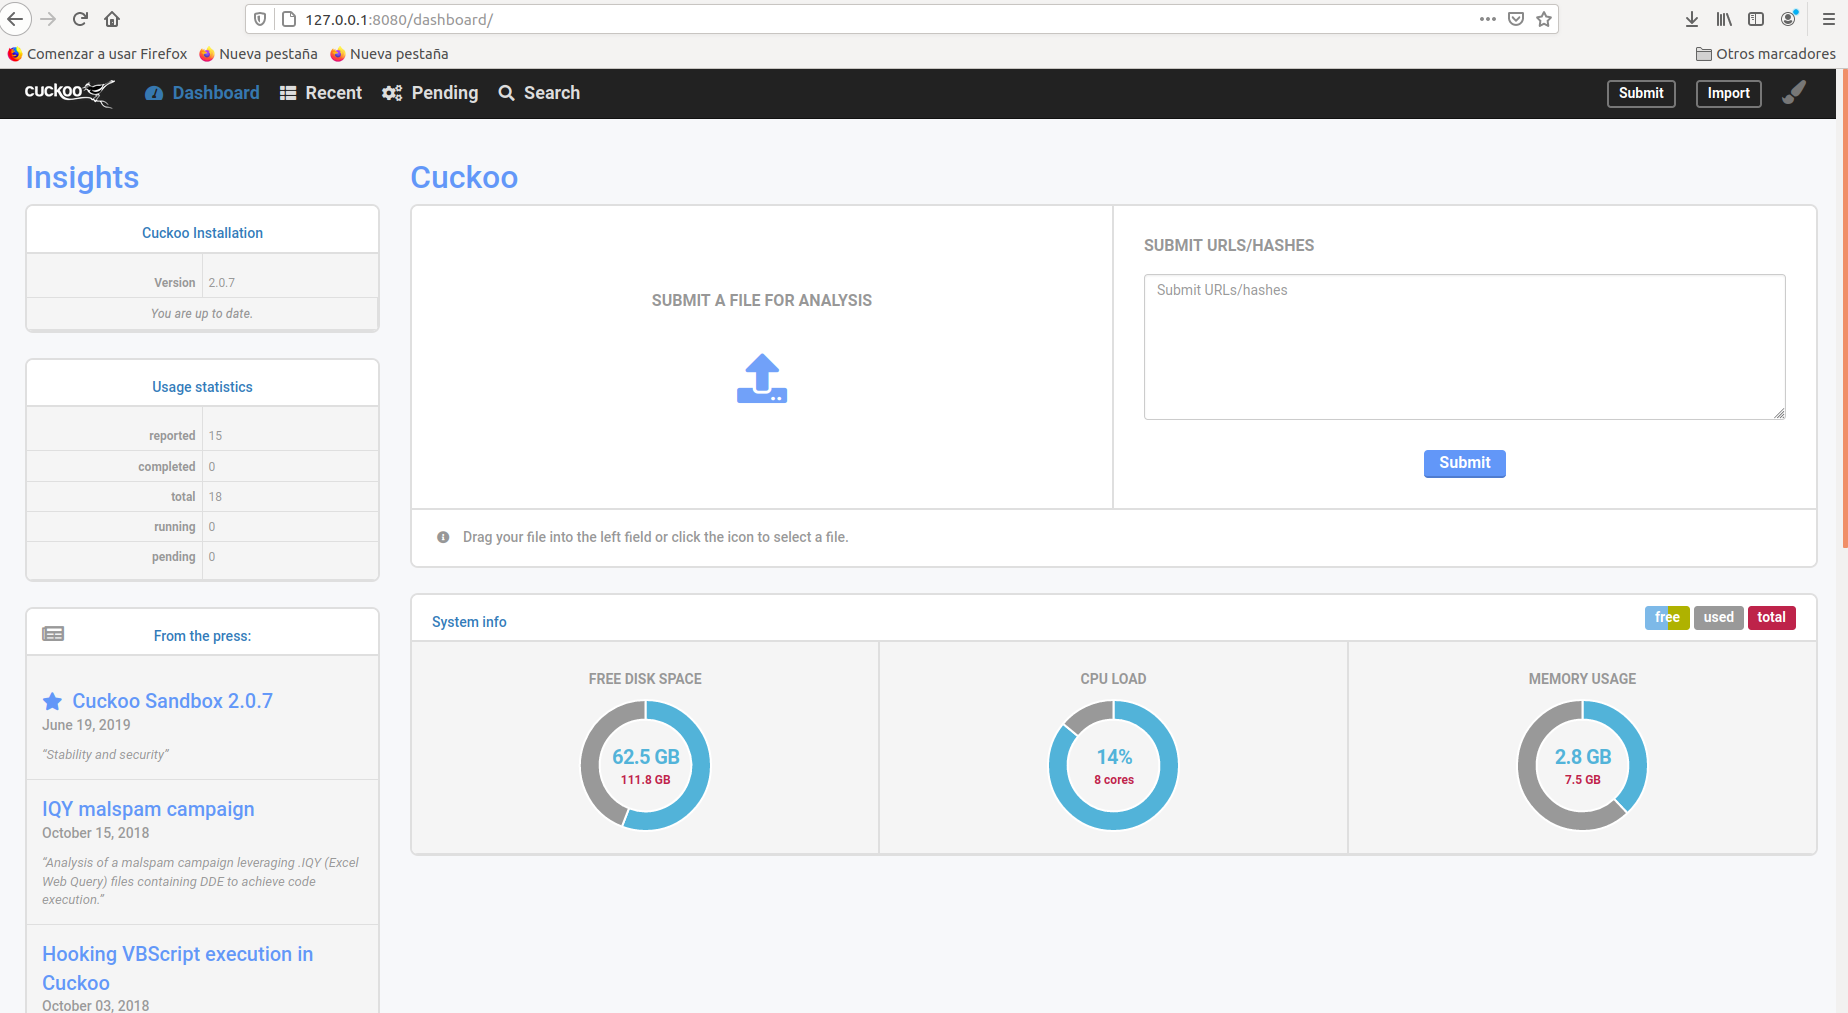
\includegraphics[width=0.9\linewidth]{images/principalcuckoo.png}
\end{center}
\caption{Pantalla principal Cuckoo Sandbox}
\label{fig:DashboardCuckoo}
\end{figure}

Al subir un archivo de malware para analizar, es posible configurar las opciones del análisis para todas las muestras o personalizar cada una. Entre las opciones, la que más interesa es la de "Internet" dentro de "Network Routing", para permitir al proceso acceder a conexión a Internet durante la ejecución. En la Figura \ref{fig:confAnalisis} se pueden observar distintas opciones de configuración.

\begin{figure}[h!]
\begin{center}
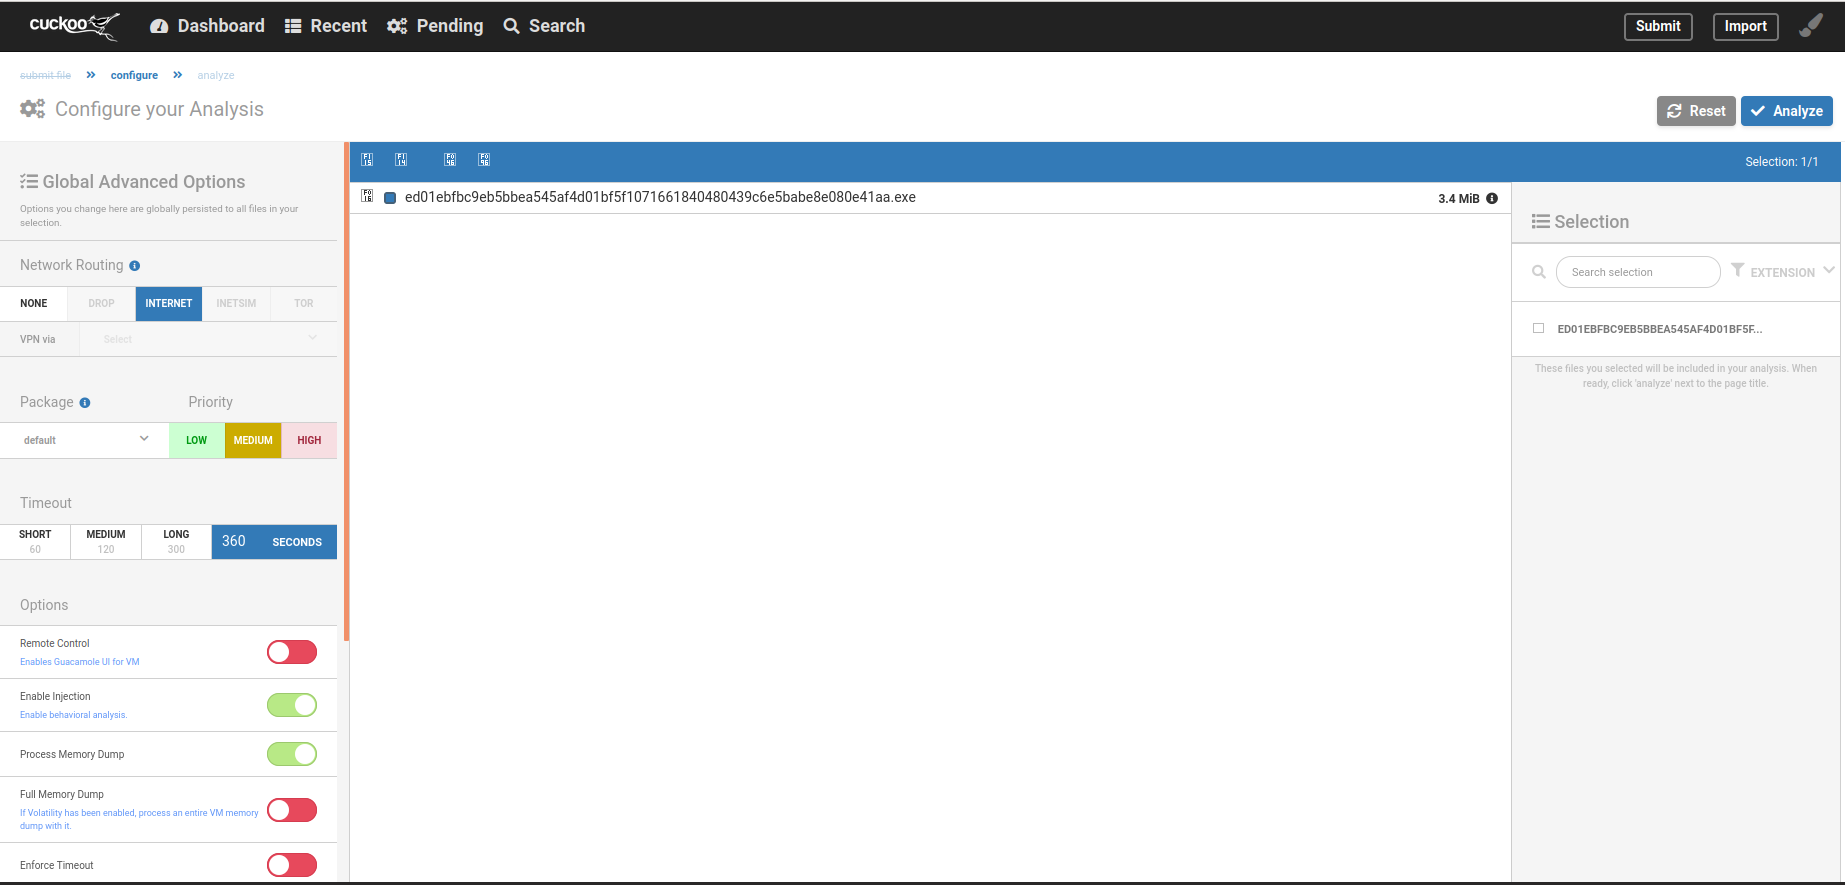
\includegraphics[width=0.9\linewidth]{images/configuracionanalisis.png}
\end{center}
\caption{Configuración del análisis}
\label{fig:confAnalisis}
\end{figure}

Después de configurar las opciones, pulsando en "Analyze" comenzará el análisis y se podrá observar cómo se abre la máquina virtual de Windows 7 y comienza la ejecución, viendo en todo momento qué va ocurriendo. Si se decide cambiar la configuración de Cuckoo para que no aparezcan las máquinas virtuales, no se podrá observer el comportamiento en directo de la muestra pero al haber instalado la herramienta "pillow" en las máquinas virtuales, se realizarán capturas de pantalla de lo que está ocurriendo.

En las Figuras \ref{fig:avisomalware} y \ref{fig:pagorescate}, se pueden observar capturas de pantalla realizadas durante el proceso de análisis que muestran un aviso de equipo infectado y una pantalla de instrucciones para el pago del rescate por la encriptación.

\begin{figure}[h!]
\begin{center}
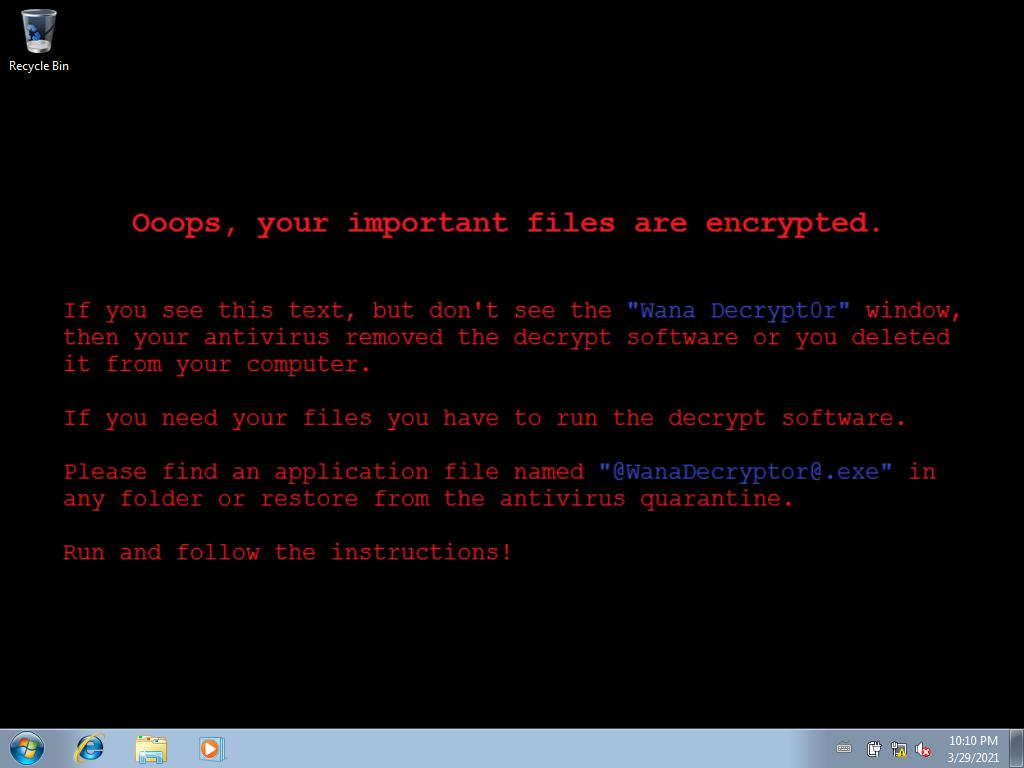
\includegraphics[width=0.72\linewidth]{images/wannacry1.jpg}
\end{center}
\caption{Aviso de malware}
\label{fig:avisomalware}
\end{figure}

\begin{figure}[h!]
\begin{center}
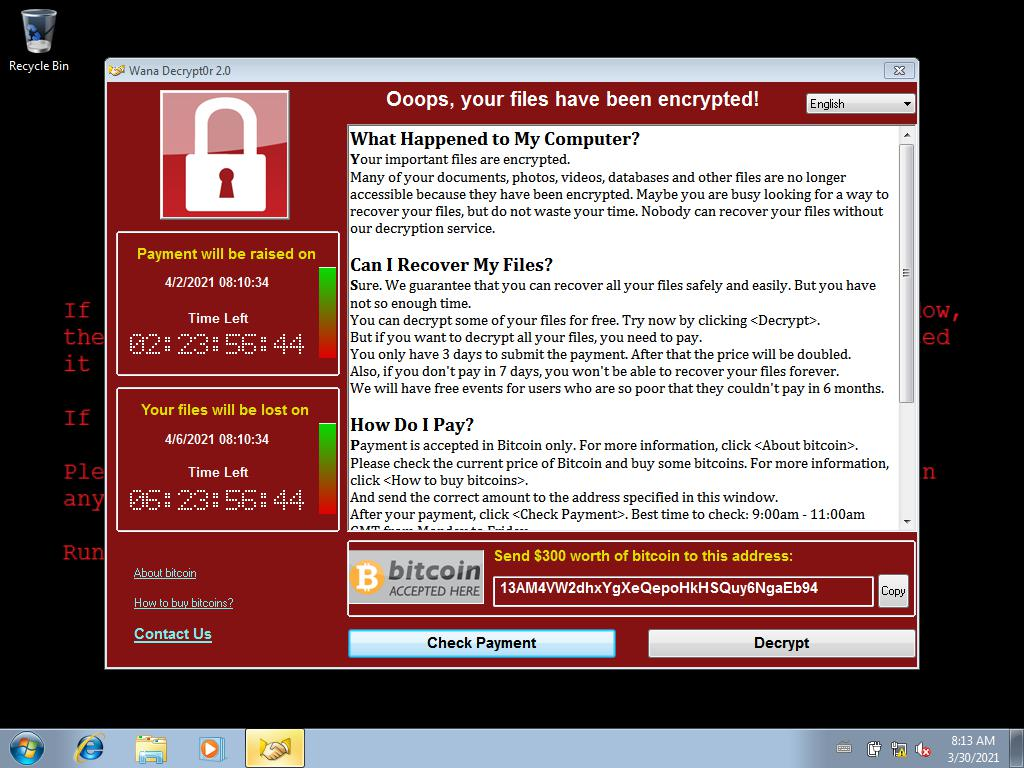
\includegraphics[width=0.72\linewidth]{images/wannacry2.jpg}
\end{center}
\caption{Pantalla de pago del rescate}
\label{fig:pagorescate}
\end{figure}

Al terminar, la máquina virtual se cerrará y en el navegador se podrán visualizar los resultados del análisis, con la puntuación obtenida, detalles técnicos sobre la muestra, capturas de pantalla, información sobre los eventos y su peligrosidad y un menú lateral para acceder a distintas características, entre otras cosas, tal y como se muestra en las Figuras \ref{fig:resulanalisis1} y \ref{fig:resulanalisis2}.

\begin{figure}[h!]
\begin{center}
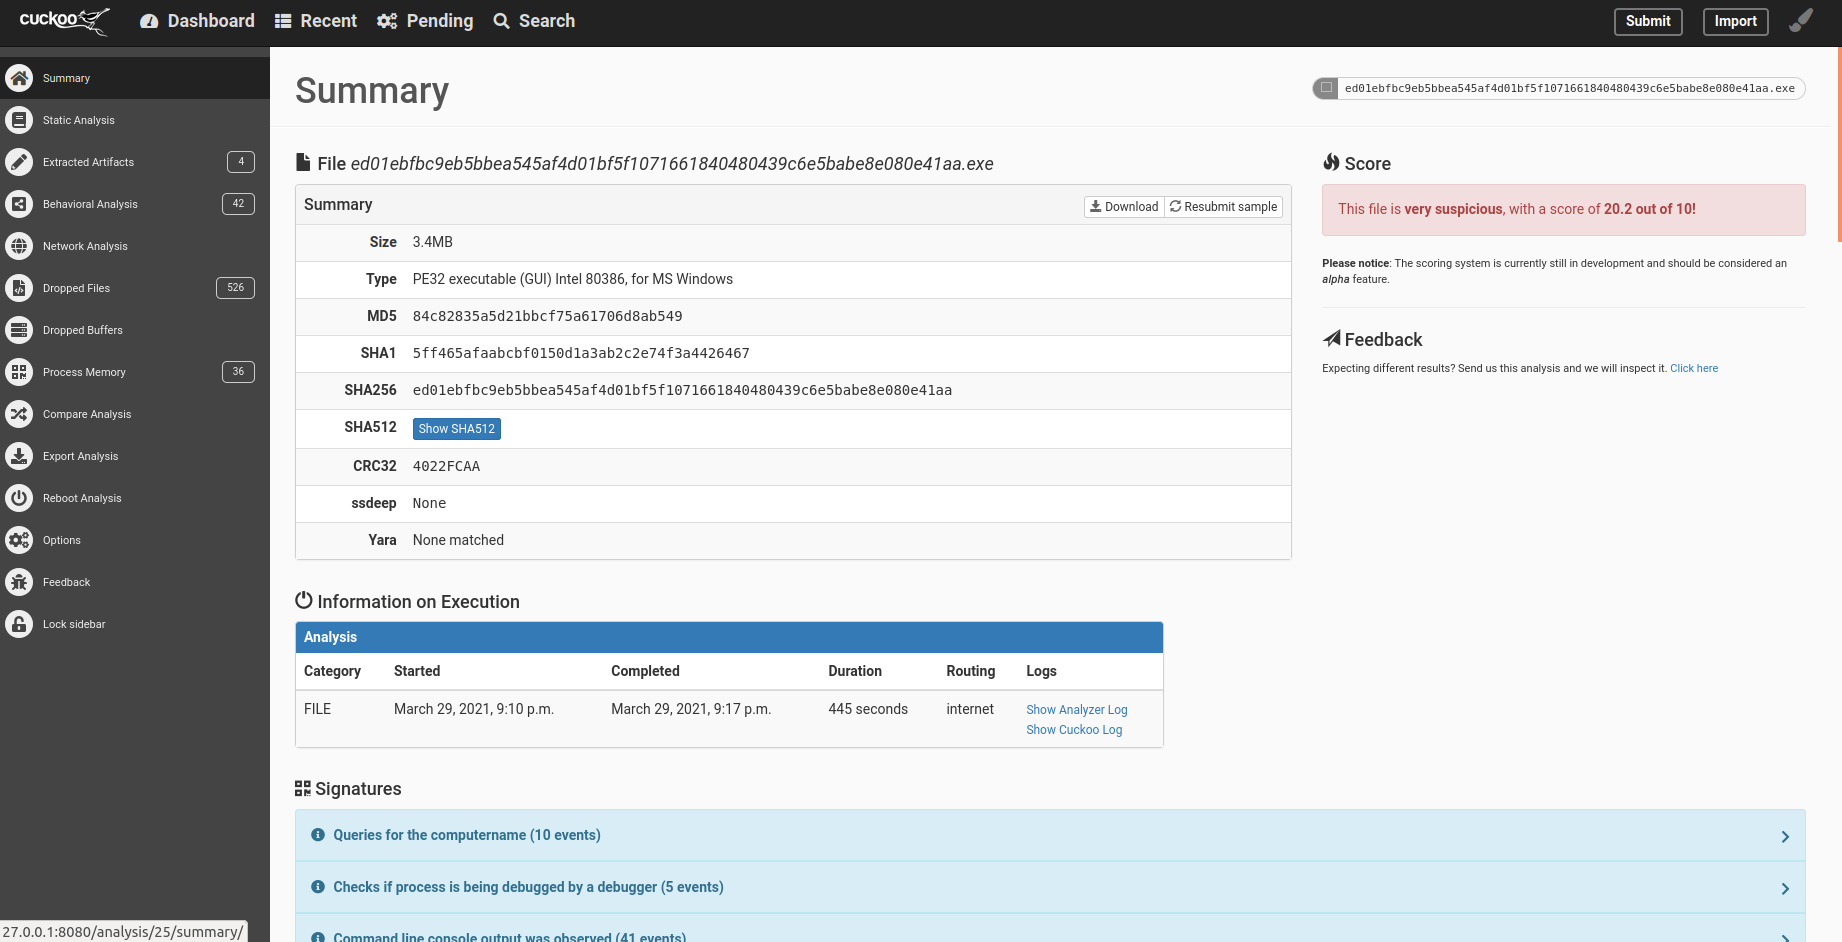
\includegraphics[width=0.9\linewidth]{images/resultadosanalisis1.png}
\end{center}
\caption{Resultados de análisis 1}
\label{fig:resulanalisis1}
\end{figure}

\begin{figure}[h!]
\begin{center}
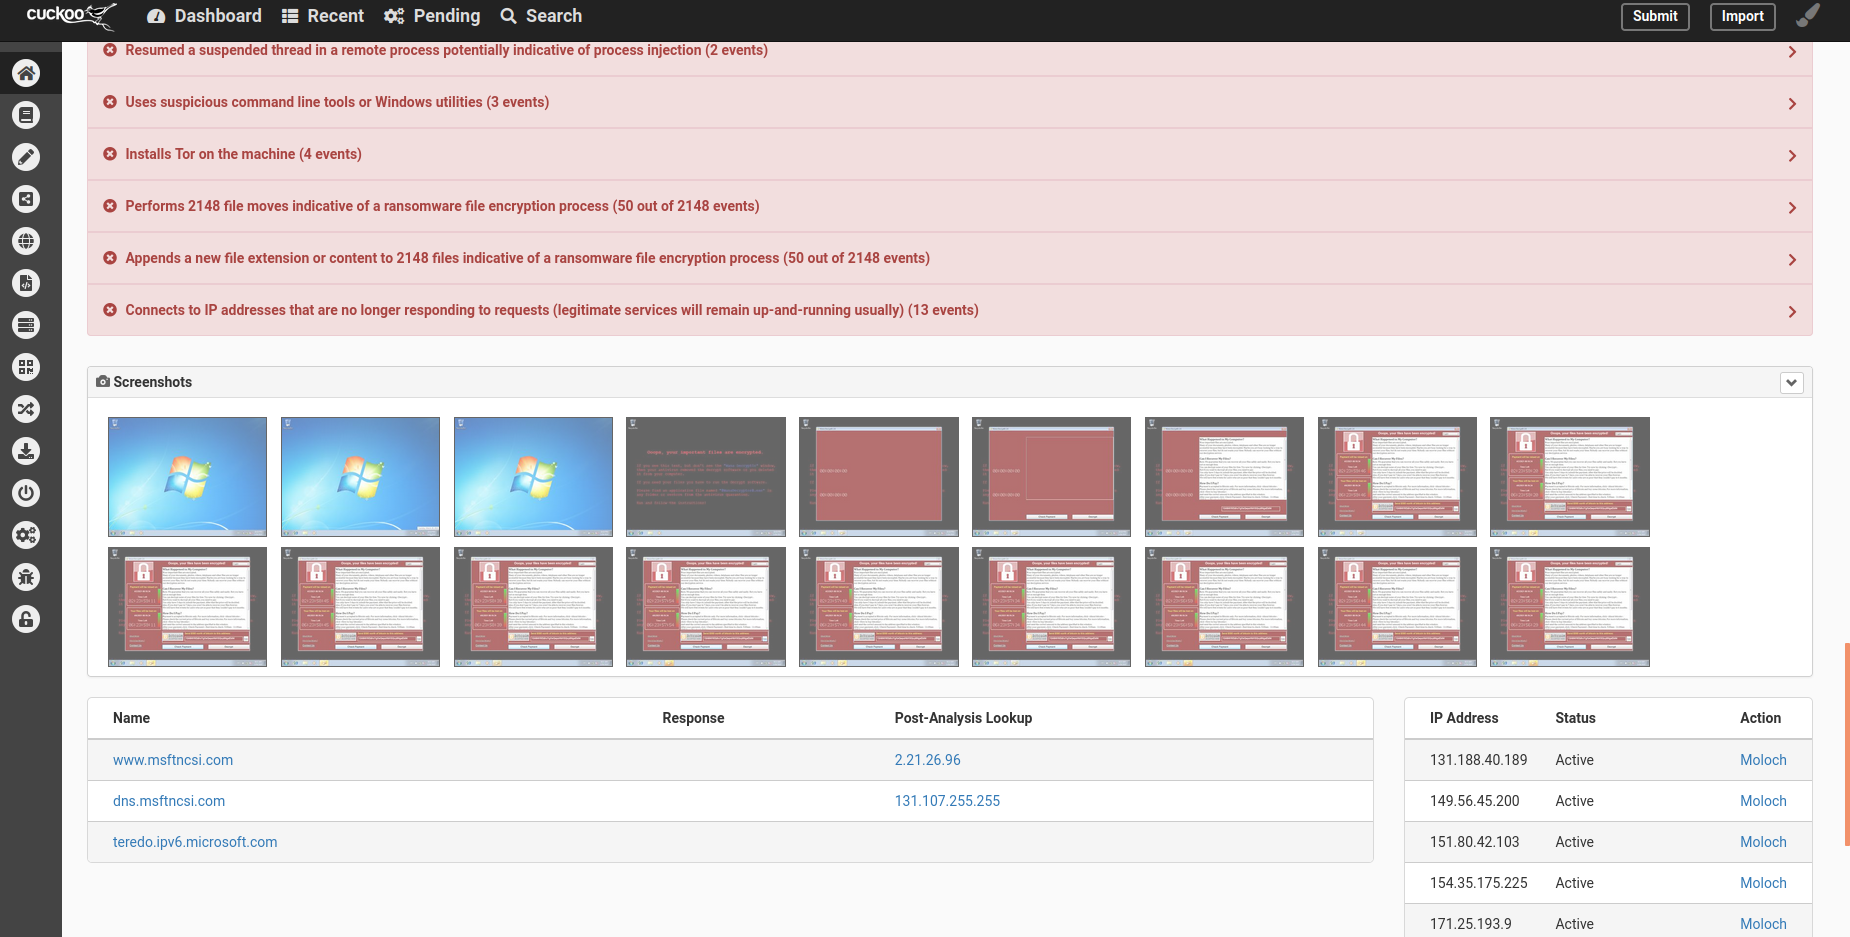
\includegraphics[width=0.9\linewidth]{images/resultadosanalisis2.png}
\end{center}
\caption{Resultados de análisis 2}
\label{fig:resulanalisis2}
\end{figure}

Toda esta información que se encuentra en la interfaz web, estará también en la carpeta ``storage'' dentro del directorio principal de trabajo de Cuckoo, organizada por carpetas para cada muestra, y repartida en sus correspondientes archivos de extensión ``.log'', ``.json'', ``.pcap''...



%SECCION DE HERRAMIENTAS/LIBRERIAS/PAQUETES QUE HEMOS USADO

\section{Conformación del \textit{Dataset}} \label{sec:reports}

\noindent En esta sección se explica cómo se ha formado el \textit{dataset} a partir de los datos obtenidos del entorno de laboratorio con Cuckoo Sandbox instalado, descrito en la Sección \ref{sec:dataset}.

\subsection{Estructura de reportes}

\noindent Cuando se realiza el análisis de muestras de ransomware, los resultados obtenidos y los informes generados se guardan en carpetas nombradas con un identificador generado automáticamente por Cuckoo Sandbox en el directorio ``\verb!/storage/analyses/!'' dentro del directorio principal de trabajo de la herramienta. La estructura de la información generada sigue aproximadamente el siguiente esquema:

\begin{listing}[style=consola, numbers=none]
.
|-- analysis.log
|-- binary
|-- dump.pcap
|-- memory.dmp
|-- files
|   |-- 1234567890_dropped.exe
|-- logs
|   |-- 1232.bson
|   |-- 1540.bson
|   `-- 1118.bson
|-- reports
|   |-- report.html
|   |-- report.json
`-- shots
    |-- 0001.jpg
    |-- 0002.jpg
    |-- 0003.jpg
    `-- 0004.jpg
\end{listing}

De todos los archivos que genera Cuckoo Sandbox, se hace hincapié en el fichero ``\verb!report.json!'', que contiene todo lo generado por el análisis divido por secciones según la información que contengan, tal y como se muestra en el siguiente esquema \cite{CKRPRT}:

\begin{listing}[style=consola, numbers=none]
report
|-- info
|-- signatures
|-- target
|-- shots
|-- static
|-- dropped
|-- behavior
|-- debug
|-- metadata
|-- screenshots
|-- strings
|-- network
`-- virustotal
\end{listing}


De todas las secciones anteriores, se presta especial atención a ``\verb!behavior!'', que muestra todo lo relacionado con los procesos ejecutados por el malware durante su actuación, el orden de los procesos, el comportamiento, las interacciones con el sistema, las llamadas a \gls{API}s de Windows, etc., y a ``\verb!signatures!'', que contiene las firmas que han dado un resultado positivo en el análisis, y sirven para identificar patrones o comportamientos concretos personalizados ya que Cuckoo Sandbox ofrece la posibilidad de crear firmas u obtener firmas creadas por otros usuarios de la comunidad \cite{CKRPRT} \cite{CKDOC}. 


\subsection{Limpieza y Extracción de Características} \label{sec:features}

\noindent En los ficheros proporcionados por el Grupo de Investigación \cite{GASS01} con resultados de análisis de muestras de \textit{ransomware} y muestras de \textit{goodware} se encuentra información variada como la puntuación del análisis, una lista \gls{API}s o información de red (\textit{pcaps}), entre otros. Se realiza una limpieza de los datos, dejando únicamente la lista de \gls{API}s y la lista de \textit{signatures}, que será la información necesaria para componer el \textit{dataset} final.

En cuanto a los informes generados por los análisis de muestras realizados en el laboratorio construido en este proyecto, se hará uso del fichero ``\verb!report.json!'' para obtener tanto las llamadas a \gls{API}s de Windows, que se encuentran en la sección ``\verb!apistats!'' dentro de ``\verb!behavior!'', donde para cada proceso de la ejecución, referido por su \gls{PID}, se muestran las \gls{API}s llamadas por cada uno y el número de veces que se realizan estas llamadas, como los nombres de las firmas (\textit{signatures}) del análisis, que se encuentran en la sección ``\verb!signatures!''.

Mediante un \textit{script} en Python, se analizan todos los informes de una sola vez, tanto los incluidos en el fichero de extensión .json en el cual se ha ejecutado la limpieza anteriormente mencionada, como los generados con el análisis de muestras, accediendo a la sección correspondiente para cada uno y recorriendo las llamadas a \gls{API}s, obteniendo todas las diferentes y generando un fichero \gls{CSV} con la información. 

\begin{algorithm}[htb!]
\renewcommand{\lstlistingname}{Algoritmo}
\begin{lstlisting}[language=config, caption={Pseudocódigo de análisis de informes ransomware}, captionpos=b, firstnumber=1, linewidth=14.4cm]
    Abrir y leer fichero
    Inicializar diccionario vacío

    Para cada muestra dentro del fichero json
        extraer lista de apis
        para cada api de la lista
            si la api no se encuentra en el diccionario entonces
                incluir api al diccionario

    Crear fichero csv
    Escribir cabecera

    Para cada muestra dentro del fichero
        asignar diccionario vacío
        inicializar lista de llamadas vacía
        extraer lista de apis
        para cada api de la lista
            si la api se encuentra en el diccionario vacío
                asignar cantidad de llamadas
                
        escribir lista en csv
        
    \end{lstlisting}
\label{Alg:imx}
\end{algorithm}

En cuanto a la representación del fichero de extensión \gls{CSV} generado en el análisis de los reportes, la primera de las columnas se utiliza para identificar cada informe mediante el listado de las \textit{signatures} del informe generado, la siguiente, determinará si se trata de una muestra ransomware o una muestra benigna y, el resto de columnas se corresponden con las 302 diferentes \gls{API}s únicas que se han obtenido en el análisis de los informes recogidos. En cuanto a las filas, cada una de ellas corresponde a una muestra representando de manera binaria en sus celdas, si la \gls{API} correspondiente ha sido llamada durante el proceso de ejecución o no.

Una vez construido el fichero \gls{CSV}, compuesto por 15352 filas, de las cuales 5456 corresponden a muestras \textit{ransomware} y 10896 a muestras \textit{goodware}, se procede a una limpieza de datos en dos pasos. En el primer paso se eliminan las filas cuyo identificador (compuesto por la lista de firmas (\textit{signatures})) se encuentre repetido, eliminando las muestras que realicen el mismo patrón de firmas y obteniendo 5416 filas \textit{ransomware} y 9648 filas \textit{goodware}. En el segundo paso, considerando que las muestras que hacen uso de las mismas funciones tienen un comportamiento y objetivos similares, se eliminan las filas idénticas en cuanto a llamadas a \gls{API}s, buscando la mayor heterogeneidad posible del conjunto de datos y evitando el \textit{overfiting} (el sobreentrenamiento de los datos, lo que refuerza comportamientos concretos del modelo). Con esta limpieza, el resultado obtenido es de 1596 filas \textit{ransomware} y 357 filas \textit{goodware}.

Tras la limpieza, el número de filas \textit{ransomware} supera ampliamente al resto, por lo que para equilibrar el \textit{dataset}, se escogen aleatoriamente 357 filas de este tipo de muestras para que no existan sesgos en los datos por la presencia predominante de un tipo de muestras. Realizado este proceso, el \textit{dataset} que se utilizará para alimentar el modelo de \gls{ML} estará compuesto de 714 filas, correspondiendo la mitad a muestras \textit{ransomware} y la otra mitad a muestras \textit{goodware} y teniendo la misma representación detallada anteriormente, con la excepción de que existirá una primera columna con un número entero identificador único que es asignado a cada fila durante la limpieza de los datos. Este \textit{dataset} se denomina \textit{dataset binario}.

Debido a la gran reducción de datos ocasionada por la limpieza y a la intención de ampliar la investigación, se decide formar un segundo \textit{dataset} siguiendo las mismas pautas y empleando las mismas técnicas aplicadas anteriormente con la diferencia de que esta vez, además de reflejar las llamadas por cada muestra a las diferentes \gls{API}s, se detallará el número de veces que éstas han sido invocadas, por lo que ya no es necesario eliminar las filas idénticas en cuanto a llamadas a \gls{API}s.

Siguiendo estos pasos, el segundo \textit{dataset} tendrá un total de 6630 filas, correspondiendo cada mitad (3315) a muestras \textit{ransomware} y \textit{goodware} respectivamente, lo que supone una cantidad considerablemente mayor respecto a la primera limpieza de datos realizada. Este segundo \textit{dataset} se denomina \textit{dataset suma}.

La Tabla \ref{tab:datasetsfin} muestra el nombre, distribución y tamaño de los \textit{datasets} finales que se usarán para alimentar el modelo de \gls{ML}.

\begin{table}[htb!]
\centering
\scriptsize %para hacer la tabla mas pequeña
\caption{\textit{Datasets} finales.}
\begin{tabular}{|c|c|c|}
\hline
\rowcolor[HTML]{C0C0C0}
\multicolumn{1}{|c|}{\cellcolor[HTML]{C0C0C0}{\textbf{Nombre}}} & \multicolumn{1}{c|}{\cellcolor[HTML]{C0C0C0}{\textbf{Distribución}}} & 
\multicolumn{1}{|c|}{\cellcolor[HTML]{C0C0C0}{\textbf{Tamaño}}} \\ \hline
    \textbf{\textit{Dataset binario}} & 357 muestras de ransomware y 357 muestras de goodware & 714 muestras \\ \hline
    \textbf{\textit{Dataset suma}} & 3315 muestras de ransomware y 3315 muestras de goodware & 6630 muestras\\ \hline
\end{tabular}
\label{tab:datasetsfin}
\end{table}






\section{Modelo y Algoritmos} \label{sec:model}
\noindent En esta sección se exponen el modelo de \gls{ML} utilizado para la clasificación del ransomware, así como los diversos algoritmos empleados para ello. 
Para desarrollar un modelo adecuado para el problema es preciso seguir una serie de pasos \cite{MLMODEL2019} \cite{Thomas_2020}:

\begin{enumerate}
    \item \textbf{Definición del problema}: Es necesario conocer si existe una solución para el problema, y si las salidas se podrán predecir con una serie de entradas proporcionadas. Se debe tener claro que el \gls{ML} se utiliza para memorizar pautas en los datos, por lo que solo se podrá obtener soluciones a problemas similares al entrenamiento realizado. En el caso de este proyecto, el problema se define como la clasificación de muestras ejecutables en benignas y ransomware.
    
    \item \textbf{Recopilación de los datos}: En esta fase se recogen todos los datos que vayan a ser usados para formar el \textit{dataset} del modelo y se dividen en datos de entrenamiento y datos de prueba. Los primeros serán los utilizados para construir el modelo y los últimos para evaluar el mismo. Se trata de un proceso crítico, puesto que los datos de entrada constituyen el combustible principal para el funcionamiento correcto del modelo. La obtención de los datos se explica con detalle en la Sección \ref{sec:dataset}.
    
    \item \textbf{Elección de indicadores de éxito}: Las métricas o indicadores son imprescindibles para conocer el funcionamiento y los resultados del modelo, de forma que se puedan introducir cambios para superarlos. En el caso de este estudio se escogen la precisión (\textit{accuracy}), exactitud (\textit{precision}), exhaustividad (\textit{recall} o \gls{TPR}), valor-F (\textit{f1-score}), la tasa de error, \gls{TNR}, \gls{FPR} y \gls{FNR}, explicadas con mayor detalle en la Sección \ref{sec:metricas}.
    
    \item \textbf{Establecimiento de protocolo de evaluación}: La validación cruzada permite estimar la capacidad de predicción de un modelo, evaluando el rendimiento de los algoritmos de aprendizaje automático que se utilizan \cite{automatic}. Se basa en la división de las muestras en un conjunto de entrenamiento para entrenar el modelo y un conjunto de pruebas para evaluarlo. La Figura \ref{fig:kfold} muestra el funcionamiento de la validación cruzada K-Fold \cite{6226477}.
    
    \begin{figure}[htb]
    \begin{center}
    {\scalebox{.68}{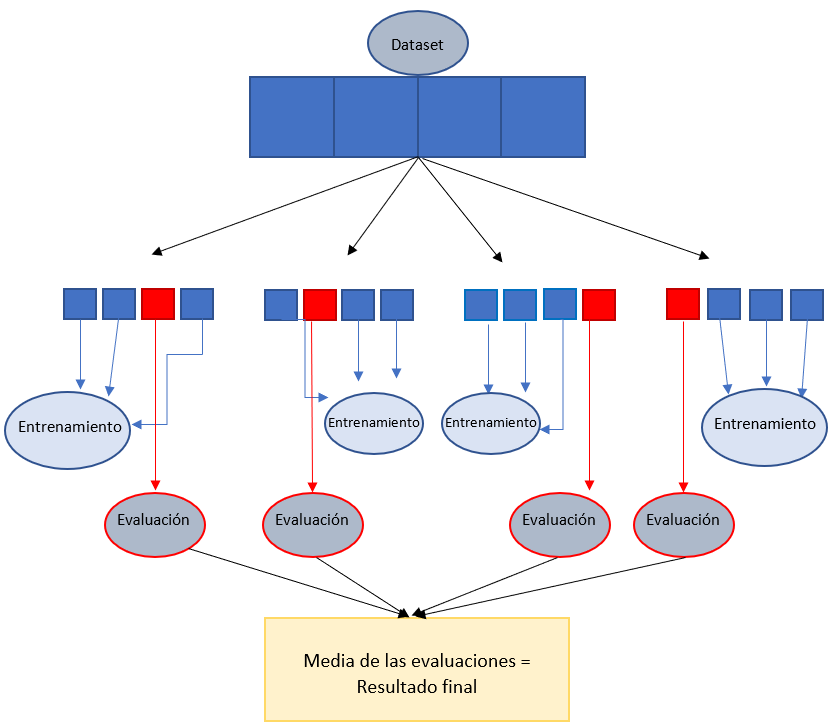
\includegraphics{images/kfold.png}}}
    \end{center}
    \caption{Funcionamiento de la validación cruzada K-Fold}
    \label{fig:kfold}
    \end{figure}
    
    En esta validación, el conjunto de muestras se divide aleatoriamente en K subconjuntos de igual tamaño. El entrenamiento se realiza con un subconjunto k-1, y el subconjunto restante se emplea para probar los datos. Este proceso se repite k veces para que cada uno de los k subconjuntos se use una vez como datos de prueba. Los resultados de cada iteración se promedian para estimar el rendimiento del modelo \cite{151}. Este trabajo utiliza el método de validación \textit{k-Fold}, en el cual el \textit{dataset} se divide de manera aleatoria en k subconjuntos. Uno de estos subconjuntos se emplean para el test como datos de validación, mientras que los k-1 restantes conforman los datos de entrenamiento. Los k resultados obtenidos son ponderados para proporcionar un único resultado.
    
    
    \item \textbf{Preparación de los datos}: Es necesario procesar los datos antes de introducirlos al modelo, por lo que se debe realizar una limpieza para obtener un formato adecuado: eliminar campos vacíos, despreciar muestras insignificantes, eliminar filas repetidas, etc. Para ello, será necesario aplicar una serie de operaciones de transformación sobre ellos. Se emplean operaciones como la normalización, la estandarización o la aplicación de expresiones no lineales. Es preciso que los datos sean del mismo tipo, y deben ser datos categóricos, transformando los datos a enteros, por ejemplo mediante codificación ``one hot'' que se aprecia en la Figura \ref{fig:onehot}. 
    
    \begin{figure}[h!]
    \begin{center}
    {\scalebox{.625}{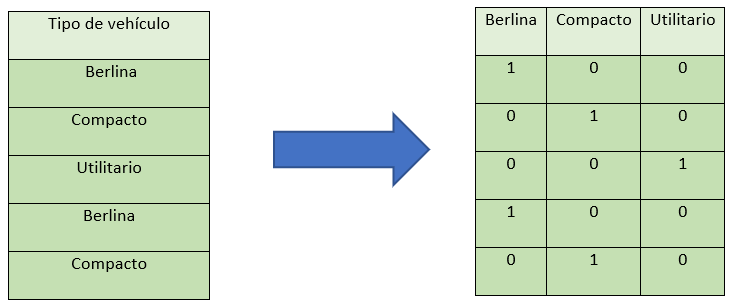
\includegraphics{images/one_hot.png}}}
    \end{center}
    \caption{Codificación one hot}
    \label{fig:onehot}
    \end{figure}
    
    \item \textbf{Extracción de características}: El \textit{dataset} utilizado puede tener ciertas características que no sean importantes para el modelo, por lo que se seleccionaran las necesarias para implementar el modelo de forma que no haya variables redundantes que perjudiquen la precisión del modelo y se obtenga la mayor eficiencia. Se trata de un proceso de vital importancia, que junto a las pautas anteriores para la preparación de los datos, ayuda a reducir el \textit{overfitting}, un mal funcionamiento del modelo debido a la redundancia de los datos. La extracción de características llevada a cabo en el proyecto se detalla en la Sección \ref{sec:features}.
    
    \item \textbf{Selección del modelo}: Dependiendo del tipo de datos se vayan a utilizar y la finalidad del modelo, se elegirá un modelo de \gls{ML} u otro, ya que existen diversos tipos y cada uno es más adecuado a un tipo de datos o forma de trabajo. Por ejemplo, los modelos de regresión están más destinados a tratar variables continuas.
    
    \item \textbf{Desarrollo del modelo}: El objetivo es crear un modelo de comparación, para medir el rendimiento de los diferentes algoritmos para obtener el mejor resultado posible y más ajustado. En este estudio se han utilizado los siguientes algoritmos: \gls{SVM} tanto con kernel \gls{RBF} como lineal, \gls{NB}, \gls{KNN}, \gls{LR}, \gls{DT} y \gls{RF}, explicados en mayor profundidad en la Sección \ref{sec:algoritmos}.
    
    \item \textbf{Prueba del modelo}: En esta fase, se prueba el modelo entrenado con los datos seleccionados y se obtienen los resultados correspondientes.
    
\end{enumerate}


%Hablar de la libreria utilizada:scikit, matplotlib para generar los graficos...

Para el desarrollo del modelo y los experimentos, se utiliza el lenguaje de programación Python y se hace uso principalmente de la librería de \gls{ML} ``scikit-learn'' \cite{scikit-learn}. Esta librería \textit{open source} proporciona herramientas simples y eficientes para el análisis predictivo de datos. Su diseño permite la interoperabilidad con la librería matemática NumPy, que proporciona gran capacidad de cómputo numérico en Python. 
Una vez obtenidos los resultados, se emplea la librería ``matplotlib'' \cite{matplotlib} para mostrar de manera gráfica el comportamiento del modelo, que posibilita la creación de figuras y esquemas de gran precisión totalmente adaptables.  

